\chapter{Reciever structure}

\section{Basic receiver structure}
\label{basic_rev_struct}
A basic general receiver structure can be seen on \autoref{fig:basic_receiver_structure}. It consists of the most common blocks in a receiver, because of the block form it is possible to separate and analyse each block individually. 

\begin{figure}[H]
\centering
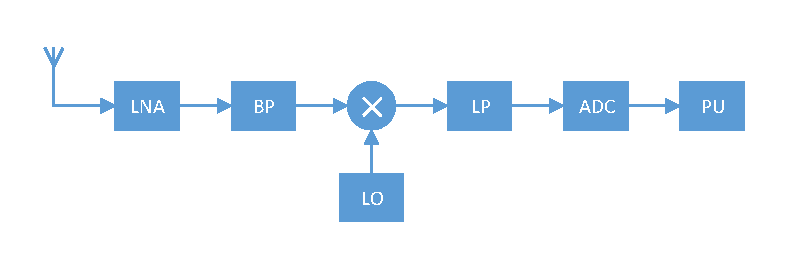
\includegraphics[width= \textwidth]{figures/Receiver.pdf}
\caption{A basic receiver structure.}
\label{fig:basic_receiver_structure}
\end{figure}

Each block will analysed with focus on the properties that could influence measurements on the fading gain i.e. gain, noise, distortion etc.

\begin{minipage}{0.48\textwidth}
\begin{itemize}
\item \textbf{Antenna}
	\begin{itemize}
	\item Emission pattern
	\item Effective gain
	\item Reflection
	\end{itemize}
\end{itemize}
\end{minipage}
\begin{minipage}{0.48\textwidth}
\begin{itemize}
\item \textbf{\Gls{LNA}}
	\begin{itemize}
	\item Gain
	\item Noise factor
	\item Distortion
	\item Saturation
	\end{itemize}
\end{itemize}
\end{minipage}
\begin{minipage}{0.48\textwidth}
\begin{itemize}
\item \textbf{\Gls{BP}}
	\begin{itemize}
	\item Phase delay/group delay
	\item Settle time
	\item Noise factor
	\item Bandwidth
	\end{itemize}	
\end{itemize}
\end{minipage}
\begin{minipage}{0.48\textwidth}
\begin{itemize}
\item \textbf{Mixer}
	\begin{itemize}
	\item Non-linearities
	\item Noise factor	
	\end{itemize}
\end{itemize}
\end{minipage}
\begin{minipage}{0.48\textwidth}
\begin{itemize}
\item \textbf{\Gls{LO}}
	\begin{itemize}
	\item Drift
		\end{itemize}
\end{itemize}
\end{minipage}
\begin{minipage}{0.48\textwidth}
\begin{itemize}
\item \textbf{\Gls{LP}}
	\begin{itemize}
	\item Phase delay/group delay
	\item Settle time
	\item Noise factor
	\end{itemize}
\end{itemize}
\end{minipage}
\begin{minipage}{0.48\textwidth}
\begin{itemize}
\item \textbf{\Gls{ADC}}
	\begin{itemize}
	\item Quantisation noise
	\item Effective number of bits
	\item Conversion time
	\end{itemize}
\end{itemize}
\end{minipage}
\begin{minipage}{0.48\textwidth}
\begin{itemize}
\item \textbf{\Gls{PU}}
	\begin{itemize}
	 \item No direct problems
	\end{itemize}
\end{itemize}
\end{minipage}


These problems can be categorized into what can be accounted for during the measurement, what can be accounted for by calibrating the equipment and what can not be easily dealt with.

\begin{itemize}
\item Avoidable problems
	\begin{itemize}
	\item Settle time
	\item Saturation
	\end{itemize}
\item Calibration problems
	\begin{itemize}
	\item Reflection
	\item Gains
	\item Phase delay/ group delay
	\item Drift
	\item Non-linearities
	\item Effective number of bits
	\end{itemize}
\item Statistical problems
	\begin{itemize}
	\item Noise
	\item Quantization noise
	\end{itemize}
\end{itemize}

Parameters that is critical to the measurements is the BW and the antenna pattern as these two directly influence the measurement of the channel. The rest only has indirect implications on the measurements. This is supported by related work in \citep{MeasurementComplexRay}



\section{Dynamic range}
Dynamic range in RF systems is the ability of the receiver to pick out weak signals compared to the strong ones(the range of the low signals to the high signals which the receiver can operate). Think about it as trying to hear a person talking when somebody in the room is screaming.  
With manual or automatic gain control,the total dynamic range of the receiver will allow it to accept a wider range of signal power.That isn't a problem as long as we want to observe the strongest signal or nearly the strongest one.The situation gets tricky when we want to observe a really weak signal in the presence of much stronger ones.That is the point where we are more interested in the instantaneous dynamic range.
The instantaneous dynamic range is specified as the difference between the strongest to the weakest signal(in dB) that can be present in a receiver's pass band while the receiver is meeting full specified performance in receiving and processing the weaker signal.
The maximum strength that a receiving system can accept and process depends on the sensitivity of the receiver and it's dynamic range.
\begin{equation}
MAXstr_{dBm} = (Sens) +(DR)
\label{Max strength of a receiving system}
\end{equation}

Where MAXstr is the maximum strength of a receiving system,Sens is the sensitivity of the receiver and DR the dynamic range of the system.\citep{DyR}

Receiver sensitivity is defined as the weakest signal that can be observed and still provide a sufficient quality output.Sensitivity is determined by the sum of Thermal Noise ,Noise Figure and the Required prediction of SNR.It is normally a negative number(in dBm) and this means that a bigger number(more negative) equals a smaller signal.
The thermal noise is given by:
\begin{equation}
Noise_{dBm} = 10log(BW\cdot Te\cdot k\cdot 1000) + NF
\label{Noise1}
\end{equation}
where $BW$ is the bandwidth $Te$ is the thermal temperature and the $NF$ is the noise figure of the reviver.


\subsection{How to measure dynamic range}

In a normal receiver the dynamic range is set by the sensitivity of the receiver to the Third order intercept point. Third order intercept points are caused by over driving the receiver with too much input and that causes distortion and signal saturation. The sensitivity is more dependent on the operating environment and the receivers noise figure. \citep{understandDynamic}


\begin{figure}[H]
\centering
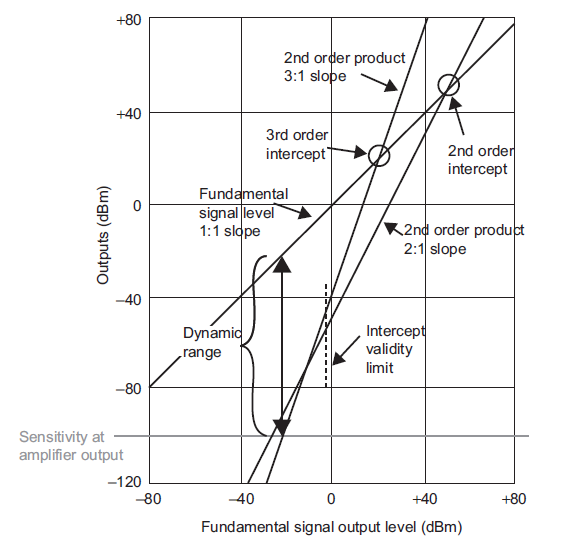
\includegraphics[width=0.90\textwidth]{figures/Dynamic_range_calc.png}
\caption{Determining the Dynamic Range from the spurs and sensitivity line.(WORK IN PROGRESS!!)}
\label{Dynamic_range_calc}
\end{figure}
 
This means that a RF receiver is highly dependent on the mixer and amplifier with regards to dynamic range. A measurement system would take into account the factors listed in \autoref{basic_rev_struct} to increase the dynamic range. Going through the \autoref{fig:basic_receiver_structure} in order from left to right. The receivers \gls{IF} is the frequency that shifted to in order to process the signal easier.  This is done in the first stages of a receiver. This frequency is normally lower than the transmitted RF frequency, this especially helps the \gls{ADC} that uses a lower sampling rate. 
By setting the \gls{IF} filter to a very narrow bandwidth (narrowband) the noise floor goes down and increases the dynamic range. 

The cost of using a narrowband is the measurement time, as the system would require a longer time for the sweep to cover a typical bandwidth. The time this would take is given by:
\todo{maybe write about averaging here and add it to the Time calculations}
\begin{equation}
T = \frac{1}{IF_{BW}} \cdot \frac{BW_{sweep}}{IF_{BW}}
\end{equation}
where $IF_{BW}$ is the intermediate frequency bandwidth and $BW_{sweep}$ is the total bandwidth you want to measure.


\subsection{Dynamic range in a VNA receiver}
\begin{figure}[H]
\centering
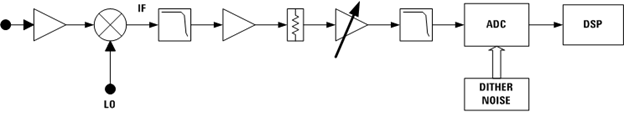
\includegraphics[width=0.90\textwidth]{figures/Block_VNA.png}
\caption{A Typical block diagram of a VNA receiver.}
\label{Block_VNA}
\end{figure}

For Network analysers the dynamic range is the maximum signal power the receiver can measure minus the noise floor of the receiver. To achieve a higher dynamic range of \gls{VNA} it must be  in tuned-receiver mode (Narrowband).
If you reduce the bandwidth then the overall noise floor will go down, so it logical that it would have higher dynamic range. \citep{AgilentNVA} \\
%%The setup of the \gls{VNA} measuring would have to take into account some factors to increase the dynamic range and still have the accuracy. Going through the \ref{Block_VNA} in order from left to right.
%%The \gls{IF} is a frequency that shifted to in order to process the signal easier. This is done in the first stages of a receiver. This frequency is normally lower than the transmitted RF frequency, this especially helps the \gls{ADC} that uses a lower sampling rate. 
%%By setting the \gls{IF} filter to a very narrow bandwidth (narrowband) the noise floor goes down and increases the dynamic range. The cost of using a narrowband is the measurement time, as the \gls{VNA} would need several sweeps to cover a typical bandwidth. \\

Dynamic range and accuracy are affected by the non-linearity in the receiver chain, the worst part are the mixers,\gls{ADC} and amplifiers since they introduce the most non-linearity. To measure the linearity of a receiver a power change measurements is preformed and compared to a reference level of power change that is accurate. This means that the linearity of a receiver as can be defined as:
\begin{equation}
Linearity = \frac{receiver \\\ measured \\\ power \\\ change}{reference \ power \ change}
\label{Linearity}
\end{equation}
 

Cross talk is the energy leakage between signal paths of the measuring system and it can be a problem in high-loss transmission measurements. This can be fixed by running an isolation calibration \citep{crosstalk}.It occurs below the noise floor so averaging and low \gls{IF} filter bandwidth must be used during calibration.
At low power levels <-70dBm the main non-linearity comes from the \gls{ADC}. Quantizing error occurs when converting from analog to digital signals. The \gls{ADC} used in \gls{VNA} are top of the line and can use a Gaussian noise ditcher to combat the non linear nature of a \gls{ADC}. 


In the digital signal processing of the \gls{VNA} averaging be applied to reduce the noise.Given the noise is uncorrelated, by averaging the measured(complex) data the noise component will approach zero.That means that our end signal in the output will be with less noise.Every time that our average is getting doubled, the signal to noise ratio is increased by 3dB. The problem is that by averaging the double of every data point the measurement will take twice as long.\citep{KeysightAVG}. The total noise floor is then given by:

\begin{equation}
Noisefloor_{dBm} = log_{2}(AVG_f)\cdot 3dB +10log(IF_{BW}\cdot T_{0}\cdot k\cdot 1000) + NF
\label{NFwithAVG}
\end{equation}
Where $IF_{BW}$ is  intermediate bandwidth $T_0$ is temperature of the system, $k$ is the Boltzmann's constant,$AVG$ is the averaging factor and $NF$ if the noise figure.
To maximise the effectiveness of a \gls{VNA} the reviver $IF_{BW}$ should be high as possible for the dynamic range needed. So to get accurate samples with the needed dynamic range in the least amount of time the $IF_{BW}$ and $AVG_f$ must be balanced to minimise time spent on one measurement.
Equipment drift is another source of error that can occur if we are operating in a place with different environmental factors for a long period of time.


\section{Diversity}
% (effects?)
Diversity is used to combat fading in a wireless system. By using clever techniques you can effectively deliver several copies or replicas of a signal to the receiver. There is a lower chance that all of these copies of signals are going to have a deep fade at the same time \citep[p. 4-6]{diversityFuture}. The overall goal is to provide a gain in signal quality by having several signals that independently fade from each other without the cost of more power consumption, reduced bit rate and complexity or other resources. There are several ways to achieve diversity in a wireless system. \\
Time diversity: By retransmitting the same information you get some diversity gain on the cost of decreased bit/rate. Usually a forward error correction code is added instead of just re transmitting the signals several times. \\
Antenna diversity / Spatial diversity
By having several antennas at both/or the receiver and transmitter a antenna diversity is achieved. With several antennas the signal can be combined together to process the signals into one. To get independently fading signals the signals need to be uncorrelated by separating the antennas least half a wavelength (micro diversity) \citep{diversityAntenna}. Antenna diversity comes at the cost of having to power more than one antenna.



